\chapter{Real numbers and sequences}
\label{sec:real_numbers_and_sequences}

\begin{notation}{The real numbers}
  The reals with be marked with a diamond. E.g., \(3.14\) would be a rational number,
  but \(\Zreal{3.14}\) is a real number.
\end{notation}

\section{Invitation: why study sequences?}
\label{sec:reals-intro}

I'm sure that you're already familiar with \textbf{sequences}. $1, 2, 3, 4, 5, \dots$
is a sequence of number that increases by one; $2, 4, 8, 16, 32, \dots$ is a sequence
of numbers which are doubling, etc. If the sequence is increasing by $d$ each time, it's an
arithmetic sequence. If it's multiplied by $r$ each time, it's a geometric sequence. It's a concept
so basic that it's already infused itself in high school algebra. So, why bother analyzing it here?

The answer is two-fold. Firstly, sequences of rationals are used to construct the reals.
Secondly, sequences are used to define limit of functions, which are the building blocks
of derivatives. We shall answer the problem of constructing the reals in this chapter,
and the limit of functions in later chapters.

The real numbers are constructed differently than all number systems prior. We can't
just introduce another operation and throw in some equivalence classes. You might say
that we can just construct rational exponentiation to get the reals, or even logarithms.
Indeed, there are infinitely many real numbers that's obtainable by rational exponentiation
and logarithms; however, there are still infinitely many more numbers which cannot be
constructed by these operations. Those numbers are called \textbf{non-algebraic numbers},
aka \textbf{transcendental numbers}. Our construction of reals must be able to capture
all these non-algebraic numbers. How? The answer is through the analysis of sequences.

Let's define what a sequence is
\begin{df}{Sequence}{reals-sequence}
  A \textbf{sequence} $a_n$ of a set $\mathbb{F}$ is a mapping $a$ from $\mathbb{N}$
  to $\mathbb{F}$.
\end{df}

\begin{notation}{}{reals-sequence}
  A sequence of a set $\mathbb{F}$ is written as $\sequence{a_n}{n = i}{f}$ where the
  starting point $i \in \mathbb{N}$ and the ending point is $f \in \mathbb{N}$. If
  $f = \infty$, then $\sequence{a_n}{n = i}{\infty}$ is an infinite sequence which starts at $i$.

  This can also be represented as a set of ordered pair
  \begin{equation}
    \sequence{a_n}{n = i}{f} = \{(i, a_i), (i + 1, a_{i+1}), \dots, (f, a_{f})\}.
  \end{equation}
\end{notation}

For example, a finite sequence of rationals, $\sequence{a_n}{n = 2}{7}$ defined as
$a_n = \frac{1}{n}$ forms the set
\begin{equation*}
  \ab\{\ab(2, \frac{1}{2}), \ab(3, \frac{1}{3}), \ab(4, \frac{1}{4}), \ab(5, \frac{1}{5}), \ab(6, \frac{1}{6}), \ab(7, \frac{1}{7})\}.
\end{equation*}
A finite sequence of rationals, $\sequence{b_n}{n = 5}{10}$, defined as $b_n = n^2$ forms the set
\begin{equation*}
  \ab\{(5, 25), (6, 36), (7, 49), (8, 64), (9, 81), (10, 100)\}.
\end{equation*}
An infinite sequence of rationals $\sequence{c_n}{n = 3}{\infty}$ defined as $c_n = n + 2$
starting at $n = 3$ is the set
\begin{equation*}
  \ab\{(3, 5), (4, 6), (5, 7), (6, 8), (7, 9), (8, 10), \dots\}.
\end{equation*}

This notation of writing ordered pairs is suggestive that the sequences form a relation.
It is a subset of \(\mathbb{N} \times \mathbb{Q}\). But it's cumbersome and doesn't do
any much good. Moving forward, we shall drop the ordered pair and just write
\begin{equation}
  \{a_i, a_{i+1}, \dots, a_f\}
\end{equation}
for the sequence \(\sequence{a_n}{n = i}{f}\) from now on.

Cauchy constructed the real numbers by saying that the real numbers are the \emph{limit}
of these \emph{converging rational sequences}. To illustrate, let's look at some
examples. Consider the sequence
\begin{gather*}
  3, 3.1, 3.14, 3.141, 3.1415, 3.14159, \dots.
\end{gather*}
This sequence, although filled with rational numbers, are \emph{gradually approaching}
the real number $\cpi$, which is not rational. Consider another sequence
\begin{equation}
  1, 1.4, 1.41, 1.4142, 1.41421, \dots.
\end{equation}
This sequence is a sequence of rationals that \emph{gradually approaches} $\sqrt{2}$.
These numbers here, $\cpi$ and $\sqrt{2}$, though not in the set of rationals, are the
number that these sequence \emph{gradually approaches}.

In math lingo, if a sequence \emph{gradually approaches} some number $L$, then that sequence is a
\textbf{convergent sequence} and $L$ is said to be the \textbf{limit} of that sequence, i.e., the
sequence converges to $L$. Here, you can clearly see how the reals can be possibly defined to
be the limit of said converging sequence. However, we quickly run into a problem.

The problem with convergence is that one has to know the limit beforehand before
showing that it actually \emph{converges}. E.g., we have to know what the exact
value of $\cpi$ in order to show that the sequence
\begin{equation*}
  3, 3.1, 3.14, 3.141, 3.1415, 3.14159, \dots
\end{equation*}
is actually a convergence sequence in the first place. I.e., we want to construct the
reals by using the limit of a rational sequence, but we need to know what the reals are
in order to show that the sequence actually converges. This is circular reasoning, and
is undesirable in mathematics. To break out of this reasoning loop, we must show that
a sequence of rational converges without knowing its limit in the first place.

Cauchy's constructed the reals by showing that all convergent sequences are Cauchy
sequence. Informally,
\begin{displayquote}
  \emph{A Cauchy sequence is a sequence whose elements become arbitrarily close to each
  other as the sequence progresses.}
\end{displayquote}
After which, the algebraic operations on the reals will then be defined as the
operation on each term of the sequence. E.g., if the real $x$ is defined as the
limit of the sequence $\sequence{a_n}{n = i}{\infty}$ and the real $y$ as the limit
of the sequence $\sequence{b_n}{n = i}{\infty}$. Their sum can then be represented
as the limit of $\sequence{a_n + b_n}{n = i}{\infty}$, their product as the limit of
$\sequence{a_n b_n}{n = i}{\infty}$, and their ratio as the limit of
$\sequence{\frac{a_n}{b_n}}{n = i}{\infty}$, etc.

From now on, I'd like to focus on sequence of rationals because we want to construct the reals
from the rationals. So, every sequence from now on is assumed to be a rational sequence. When the
reals ($\mathbb{R}$) are finally constructed, one can replace all $\mathbb{Q}$ with $\mathbb{R}$.

\section{Cauchy sequences}

The goal of this section is for you to understand the following definition:

\begin{df}{Cauchy sequences}{reals-cauchy}
  If a rational sequence $\sequence{a_n}{n = m}{\infty}$ is Cauchy, then
  \begin{align}
    \forall (\epsilon \in \mathbb{Q}_{>0}) \exists (N \in \mathbb{N}_{>m}) \forall (j, k \in \mathbb{N}_{\geq N}) : |a_j - a_k| \leq \epsilon.
  \end{align}
\end{df}

I understand that this definition looks very unfriendly, so let's break it down and
see how each element come together to capture concept of a sequence whose elements get
closer together as the sequence progresses. In my humble opinion, the approach taken
by \citeauthor{tao-1-2022} in his \citetitle{tao-1-2022} book \cite{tao-1-2022} is one of the most
intuitive; therefore, I shall follow his teachings and deconstruct the definition of
Cauchy sequences into two bite-sized ones: $\epsilon$-steadiness and eventual $\epsilon$-steadiness.

The first definition defines what it means for \emph{two elements to be close to each other.}
\begin{df}{$\epsilon$-closeness}{reals-epsilon_closeness}
  Two numbers $a$ and $b$ are $\epsilon$-close if $|a - b| \leq \epsilon$
\end{df}
This definition measures the distance on the number line. If the distance between $a$
and $b$ is less than $\epsilon$, we say that $a$ and $b$ are $\epsilon$-close.

\begin{df}{$\epsilon$-steadiness}{reals-epsilon_steadiness}
  A rational sequence $\sequence{a_n}{n = i}{f}$ is $\epsilon$-steady if for all $j, k$
  between $i$ and $f$, $a_j$ and $a_k$ are $\epsilon$-close.
\end{df}

One interpretation of a sequence that's $\epsilon$-steady is that the range of the
sequence ($\max\ab(\sequence{a_n}{n = i}{f}) - \min\ab(\sequence{a_n}{n = i}{f})$) is
restricted to be less than or equal to $\epsilon$:
\begin{equation}
  \max\ab(\sequence{a_n}{n = i}{f}) - \min\ab(\sequence{a_n}{n = i}{f}) \leq \epsilon.
\end{equation}
Because of this, the distance between each term in an $\epsilon$-steady sequence is
always less than or equal to $\epsilon$.

This definition also works for infinite sequence. However, the concept of maxima and minima
is currently a bit loose. Sometimes, the maxima and minima doesn't even exist, so it'd
be wiser for now to think of an $\epsilon$-steady sequence as a sequence that the distance between
each and every term is less than $\epsilon$. Now, let's look at some examples and non-examples.

\begin{exmp}{$\epsilon$-steady sequences}{}
  \begin{enumerate}
    \item The sequence $\sequence{a_n}{n = 0}{\infty}$:
          $3, 3.1, 3.14, 3.141, 3.1415, 3.14159, \dots$, is $0.1$-steady but not
          $0.01$-steady, because
          \begin{equation*}
            |a_0 - a_1| = |3 - 3.1| = 0.1, \quad \textrm{which is more than} \quad 0.01.
          \end{equation*}
    \item The sequence $\sequence{b_n}{n = 0}{\infty}$: $-1, 0, 1, 0, -1, 0, \dots$ is
          $2$-steady, but not $1$-steady because
          \begin{equation*}
            |b_0 - b_2| = | - 1 - 1| = 2, \quad \textrm{which is more than} \quad 1.
          \end{equation*}
    \item The sequence $\sequence{c_n}{n = 4}{9}$: $2, 3, 1, 5, 4, 6$ is $10$-steady,
          but not $4$-steady because
          \begin{equation*}
            |c_6 - c_9| = |6 - 1| = 5, \quad \textrm{which is more than} \quad 4.
          \end{equation*}
  \end{enumerate}
\end{exmp}

Before moving on, I'd like to discuss the image of $\epsilon$-steady sequence. Consider
a sequence $\sequence{a_n}{n = 0}{\infty}$ shown in \cref{fig:reals-epsilon_steady_sequences}.
Let's draw a rectangle which infinite extends along the $x$-axis but has the height of
$\epsilon$. The sequence is $\epsilon$-steady \ifft you can find a position of this rectangle
such that every term in the sequence lies in that rectangle. Here, $\sequence{a_n}{n = 0}{\infty}$
is $\epsilon$-steady because there's a rectangle configuration in which every point of
the sequence lies in the rectangle shown in the right most figure. The left most and middle
figure doesn't count because there are some points, drawn in red, which is outside the rectangle.

\begin{figure}[]
  \centering
  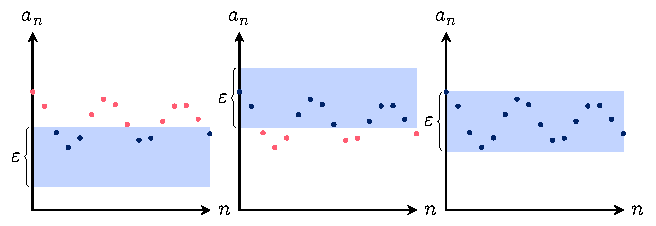
\includegraphics{realanalysis/realsandsequences/cauchysequences/epsilon-steady-sequences.pdf}
  \caption{Examples of rectangle configurations to check that a sequence is $\epsilon$-steady.}
  \label{fig:reals-epsilon_steady_sequences}
\end{figure}

The concept of a sequence being $\epsilon$-steady is quite simple, but it doesn't
capture the limiting behavior of a sequence. Since we want to construct the reals
from the \emph{limit} of a \emph{converging sequence}, we shouldn't really care about
the initial terms. Therefore, we improve on the definition of $\epsilon$-steadiness to
eventual $\epsilon$-steadiness: a definition that captures what it means for \emph{the
elements of a sequence to get close together as the sequence progresses}.
\begin{df}{Eventual $\epsilon$-steadiness}{reals-eventual_epsilon_steadiness}
  A rational sequence $\sequence{a_n}{n = i}{f}$ is eventually $\epsilon$-steady if there exists
  some natural $N \geq i$ in which the sequence $\sequence{a_n}{n = N}{f}$ is $\epsilon$-steady.
\end{df}

The intuition for this is that, if it's possible to find some number $N$ in which the
removal of the first $N$ terms of the sequence makes the sequence $\epsilon$-steady,
then the sequence is eventually $\epsilon$-steady. Let's look at some examples and non-examples.
\begin{exmp}{Eventually $\epsilon$-steady sequences}{reals-eventual_epsilon_steadiness}
  \begin{enumerate}
    \item The sequence $\sequence{a_n}{n = 1}{\infty}$:
          $1, \frac{1}{2}, \frac{1}{3}, \frac{1}{4}, \dots$, is not $\frac{1}{2}$-steady because
          \begin{equation*}
            |a_0 - a_2| = \ab|1 - \frac{1}{3}|
                        = \frac{2}{3}, \quad \textrm{which is more than} \quad \frac{1}{2};
          \end{equation*}
          however, the sequence is eventually $\frac{1}{2}$-steady because the removal
          of the first term yields a sequence that is $\frac{1}{2}$-steady:
          \begin{equation*}
            \frac{1}{2}, \frac{1}{3}, \frac{1}{4}, \frac{1}{5}, \dots,
          \end{equation*}
    \item The sequence $\sequence{b_n}{n = 0}{\infty}$:
          $1, \frac{1}{2}, \frac{1}{4}, \frac{1}{8}, \dots$, is not $\frac{1}{4}$-steady because
          \begin{equation*}
            |a_2 - a_4| = \ab|\frac{1}{2} - \frac{1}{8}|
                        = \frac{3}{8}, \quad \textrm{which is more than} \quad \frac{1}{4};
          \end{equation*}
          however, the sequence is eventually $\frac{1}{4}$-steady because the removal
          of the first two terms yields a sequence that is $\frac{1}{4}$-steady:
          \begin{equation*}
            \frac{1}{4}, \frac{1}{8}, \frac{1}{16}, \frac{1}{32}, \dots.
          \end{equation*}
    \item The sequence $\sequence{c_n}{n = 0}{\infty}$: $69, 2, 2, 2, 2, \dots$ is not
          $3$-steady because for all $j > 0$,
          \begin{equation*}
            |a_0 - a_j| = |69 - 2| = 67, \quad \textrm{which is more than} \quad 3;
          \end{equation*}
          however, the sequence is eventually $3$-steady because the removal of the
          first term yields a sequence that is $3$-steady:
          \begin{equation*}
            2, 2, 2, 2, 2, \dots.
          \end{equation*}
  \end{enumerate}
\end{exmp}

And now, we're ready to define the Caychy sequences in simpler terms:
\begin{cor}{Cauchy sequences}{reals-cauchy_sequences_redefined}
  A Cauchy sequence is an infinite sequence which is eventually \(\epsilon\)-steady for all
  $\epsilon > 0 \in \mathbb{Q}$. I.e., for a sequence $\sequence{a_n}{n = m}{\infty}$ to be Cauchy,
  \begin{equation*}
    \forall (\epsilon \in \mathbb{Q}_{>0}) \exists (N \in \mathbb{N}_{>m}) \forall (j, k \in \mathbb{N}_{>N}) : |a_j - a_k| \leq \epsilon
  \end{equation*}
\end{cor}

A natural question to ask is then \emph{how to prove that a sequence is Cauchy?} It
is quite hard to grasp, and it's possibly one of the first major roadblocks in learning real
analysis. But at least, the proof is constructive and understandable. The concept is to use basic
arithmetic to show that for every $\epsilon$, there exists a corresponding $N$ which
makes the sequence $\sequence{a_n}{n = N}{\infty}$, $\epsilon$-steady. This would be
one of the first proof that must have a preparation stage before the actual proof.
We do some arithmetic first to decide what $N$ might be in terms of $\epsilon$, and
use that to show that for all $j, k \geq N$, the sequence is $\epsilon$-steady.

\begin{exmp}{Show that $\sequence{\frac{1}{n}}{n = 0}{\infty}$ is Cauchy}{}
  We prepare the proof by first fixing $\epsilon$ and find $N$ in terms of $\epsilon$.
  For all $n \geq N$, we demand that
  \begin{align}
    |a_j - a_k|                         & \leq \epsilon                                    \\
    \ab|\frac{1}{j} - \frac{1}{k}|      & \leq \epsilon                                    \\
    \ab|\frac{1}{j}| + \ab|\frac{1}{k}| & \leq \epsilon. &  & \textrm{Triangle inequality}
  \end{align}
  If we demand both $\ab|\frac{1}{j}|$ and $\ab|\frac{1}{k}|$ to be less than
  $\frac{\epsilon}{2}$, then we would get $|a_j - a_k| \leq \epsilon$ as desired; thus, let
  \begin{equation}
    \ab|\frac{1}{j}|, \ab|\frac{1}{k}| \leq \frac{\epsilon}{2}
  \end{equation}
  Since $j, k \geq N$, we have $\frac{1}{j}, \frac{1}{k} \leq \frac{1}{N}$. Combining
  this with the equation above gives
  \begin{align}
    \frac{1}{N} & \leq \frac{\epsilon}{2}  \\
    N           & \geq \frac{2}{\epsilon}.
  \end{align}
  Here, we've shown that $N \geq \frac{2}{\epsilon}$ causes $|a_j - a_k|$ where
  $j, k \geq N$ to be less than $\epsilon$ for every $\epsilon$; thus, the sequence is
  Cauchy. Now onto the formal proof.

  \begin{proof}
    \begin{align}
      |a_j - a_k|                             & = \ab|\frac{1}{j} - \frac{1}{k}|                                                 \\
      \ab|\frac{1}{j} - \frac{1}{k}|          & \leq \ab|\frac{1}{j}| + \ab|\frac{1}{k}|     &  & \textrm{Triangle's inequality} \\
      \ab|\frac{1}{j}| + \ab|\frac{1}{k}|     & \leq \frac{1}{N} + \frac{1}{N}                                                   \\
      \shortintertext{Choose $N \geq \frac{2}{\epsilon}$, then}
      \frac{1}{N} + \frac{1}{N}               & \geq \frac{\epsilon}{2} + \frac{\epsilon}{2}                                     \\
      \frac{\epsilon}{2} + \frac{\epsilon}{2} & = \epsilon.
    \end{align}
    Therefore, $N \geq \frac{2}{\epsilon}$ causes $|a_j - a_k|$ to be less than $\epsilon$
    for all $j, k \geq N$. Thus, the sequence is Cauchy.
  \end{proof}
\end{exmp}

The next example is informal but it should give you a rough idea of how you might be
able to bound these sequences. It's also a sidetrack to the proof that \(0.999\dots = 1\).

\begin{exmp}{Show that the sequence \(0, 0.9, 0.99, 0.999, \dots\) is Cauchy}{}
  Fix an \(\epsilon\), then we find \(N\) in terms of \(\epsilon\). For all \(j, k \geq N\),
  we demand that
  \begin{equation}
    |a_j - a_k| \leq \epsilon \\
  \end{equation}
  Without loss of generality, let \(j > k\), then
  \begin{align}
    |0.\underbracket{9...9}_j - 0.\underbracket{9 \dots 9}_k|  & \leq \epsilon \\
    |0.\underbracket{0...0}_{j-k}\underbracket{9 \dots 9}_{k}| & \leq \epsilon
  \end{align}
\end{exmp}

Before constructing the reals, I'd like to discuss the notion of boundedness which is
later used to prove that multiplication on the reals is well-defined

\begin{df}{Boundedness of sequences}{reals-boundedness}
  A sequence $\sequence{a_n}{n = i}{f}$ is bounded by a rational $M > 0$ if for all
  $n \in \mathbb{N}$ that's between $i$ and $f$, $|a_n| \leq M$.
\end{df}

\begin{cor}{Finite sequences are bounded}{reals-finite_sequences_bounded}
  Every finite sequence $\sequence{a_n}{n = i}{f}$ is bounded
\end{cor}
\begin{proof}
  We shall use strong induction to prove this.

  \basecase Trivially, the sequence $a_1$ is bounded by $M = |a_1|$.

  \inductivestep Assume that the sequence $\sequence{a_n}{n = i}{N}$ where $i < N < f$ is bounded
  by some rational $M$. Then, the sequence $\sequence{a_n}{n = i}{S(N)}$ must also be bounded by
  the rational $M + |a_{S(N)}|$; therefore, any finite sequence is bounded, closing the induction.
\end{proof}

The next thing is to establish a connection between Cauchy sequences and the concept of boundedness.

\begin{prop}{}{reals-boundedness-cauchy}
  Every Cauchy sequence is bounded
\end{prop}

\begin{proof}
  Since the sequence is Cauchy, for every $\epsilon$, there exists a natural $N$ such that
  for all $j, k \geq N$, $|a_j - a_k| \leq \epsilon$. The sequence can then be split into two parts:
  \begin{equation*}
    a_1, a_2, \dots, a_{N-1}, \mathand a_{N}, a_{N+1}, a_{N+2}, \dots.
  \end{equation*}
  By \cref{co:reals-finite_sequences_bounded}, the first part of the sequence is bounded
  by some rational $M$. Since the distance between every term in the second part is less than
  $\epsilon$. If the smallest term in the second part of the sequence is $K$, then the entire part
  must be bounded by $K + \epsilon$; therefore, the whole sequence is bounded by $M + K + \epsilon$.
\end{proof}

\section{Construction of the reals}

Now we are ready to construct the reals. When I said that the reals weren't an equivalent
class, I was lying a bit because it's actually an equivalence class. But it's not the equivalence
classes of the rationals. Rather, it's an equivalence class of \emph{Cauchy sequences of rationals}
as there are many Cauchy sequences which represent the same real number. I.e.,
\begin{equation}
  1, \frac{1}{2}, \frac{1}{4}, \frac{1}{8}, \frac{1}{16}, \dots, \mathand 1, \frac{1}{2}, \frac{1}{3}, \frac{1}{4}, \frac{1}{5}, \dots, \footnote{It is left as an exercise for the reader to prove that these two sequences are Cauchy.}
\end{equation}
both of which seems to approach the number $0$.

\begin{df}{Real numbers}{reals-reals}
  Two Cauchy sequences, $\sequence{a_n}{n = m_a}{\infty}$ and $\sequence{b_n}{n = m_b}{\infty}$
  are equivalent \ifft for all rational $\epsilon$, there exists a natural
  $N \geq \max(m_a, m_b)$ in which for all $n \geq N$, $a_n$ and $b_n$ are $\epsilon$-close, i.e.,
  \begin{multline}
    \forall (\epsilon \in \mathbb{Q}_{>0}) \exists \ab(N \in \mathbb{N}_{\geq \max(m_a, m_b)}) \forall (n \in \mathbb{N}_{>N}) : |a_n - b_n| \leq \epsilon
  \end{multline}
  and we write \(\sequence{a_n}{n = m_a}{\infty} \sim \sequence{b_n}{n = m_b}{\infty}\)

  A real number is an equivalence class of Cauchy sequences where we denote
  \begin{equation}
    \Zreal{x} = \ab[\sequence{a_n}{n = m_a}{\infty}]
  \end{equation}
\end{df}

The first thing to notice is that the equivalence relation defined prior does not care about the
starting point of the sequences. We analyze the equivalency for
$n \geq \max(m_a, m_b)$ only, because we only care about the behavior of the sequence
as it \emph{progresses}. Hence, for the rest of this chapter, we shall consider only
those sequences that start at zero. If it doesn't start at zero, we can always take
the maximum of the starting point and the behavior as the term progresses would still be the same.

Similar to how we've defined Cauchy sequences, we can also break
\cref{df:reals-reals} into two parts: $\epsilon$-close, and eventual
$\epsilon$-close. I shall go over them very briefly as it is analogous to how Cauchy
sequences (\cref{df:reals-cauchy}) are defined.

Two sequences $\sequence{a_n}{n = 0}{\infty}$ and $\sequence{b_n}{n = 0}{\infty}$
are $\epsilon$-close \ifft
\begin{equation}
  |a_n - b_n| \leq \epsilon
\end{equation}
and they're eventually $\epsilon$-close if there exists a natural $N > 0$ which
$\sequence{a_n}{n = N}{\infty}$ and $\sequence{b_n}{n = N}{\infty}$ are
$\epsilon$-close. Finally, these sequences are equivalence if it is eventually
$\epsilon$-close for all rational $\epsilon$.

One remark I'd like to make about the equivalence classes of the reals is that if we
don't require the sequences to be Cauchy, then there pair of sequences which aren't
Cauchy but are equivalent. E.g.,
\begin{equation}
  1, 2, 3, 4, 5, 6, \dots, \mathand 3, 3, 3, 4, 5, 6, \dots,
\end{equation}
But one interesting tangent if a sequence is equivalent to a Cauchy sequence, then it
must be Cauchy as well. Hence, the equivalence classes of Cauchy sequences are closed
--- there is no non-Cauchy sequence which is equivalent to a Cauchy sequence as seen
by the following corollary:

\begin{cor}{}{}
  Let $\sequence{a_n}{n = 0}{\infty} \sim \sequence{b_n}{n = 0}{\infty}$. If one of
  the sequence is Cauchy, then the other must also be. If one of the sequence isn't
  Cauchy, then the other is also not Cauchy.
\end{cor}

\begin{proof}
  By \cref{df:reals-reals},
  $\sequence{a_n}{n = 0}{\infty} \sim \sequence{b_n}{n = 0}{\infty}$ means
  \begin{equation}
    \forall (\epsilon \in \mathbb{Q}_{>0}) \exists \ab(N \in \mathbb{N}) \forall (n \in \mathbb{N}_{\geq N}) : |a_n - b_n| \leq \epsilon.
  \end{equation}
  Let's assume that $\sequence{a_n}{n = 0}{\infty}$ is Cauchy, i.e.,
  \begin{equation}
    \forall (\epsilon \in \mathbb{Q}_{>0}) \exists \ab(N \in \mathbb{N}) \forall (j, k \in \mathbb{N}_{\geq N}) : |a_j - a_k| \leq \epsilon. \label{eq:reals-equivalence_sequences_cauchy-1}
  \end{equation}
  We then want to prove that $\sequence{b_n}{n = 0}{\infty}$ is also Cauchy, i.e.,
  \begin{equation*}
    \forall (\delta \in \mathbb{Q}_{>0}) \exists \ab(N \in \mathbb{N}) \forall (j, k \in \mathbb{N}_{>N}) : |b_j - b_k| \leq \delta. \label{eq:reals-equivalence_sequences_cauchy-2}
  \end{equation*}
  This may seem a bit outrageous, but notice that
  \begin{equation}
    |b_j - b_k| = |b_j - a_j + a_j - a_k + a_k - b_k|.
  \end{equation}
  By the triangle's inequality, we get
  \begin{equation}
    |b_j - a_j + a_j - a_k + a_k - b_k| \leq |b_j - a_j| + |a_j - a_k| + |a_k - b_k|.
  \end{equation}
  From \cref{eq:reals-equivalence_sequences_cauchy-1,eq:reals-equivalence_sequences_cauchy-2},
  \begin{equation}
    |b_j - a_j| + |a_j - a_k| + |a_k - b_k| \leq 3 \epsilon,
  \end{equation}
  or $|b_j - b_k| \leq 3\epsilon$. If $\delta = 3\epsilon$, then $|b_j - b_k| \leq \delta$
  as desired.
\end{proof}

Now we shall prove that the relation defined in \cref{df:reals-reals} are equivalence relations.

\begin{prop}{The defining relation of the reals is an equivalence relation}{}
  Let \(\sequence{a_n}{n = 0}{\infty}\), \(\sequence{b_n}{n = 0}{\infty}\), and
  \(\sequence{c_n}{n = 0}{\infty}\) be Cauchy sequences of the rationals, then
  \begin{itemize}
    \item \(\sequence{a_n}{n = 0}{\infty} \sim \sequence{a_n}{n = 0}{\infty}\)
    \item \(\ab(\sequence{a_n}{n = 0}{\infty} \sim \sequence{b_n}{n = 0}{\infty}) \implies \ab(\sequence{b_n}{n = 0}{\infty} \sim \sequence{a_n}{n = 0}{\infty})\)
    \item \(\ab[\ab(\sequence{a_n}{n = 0}{\infty} \sim \sequence{b_n}{n = 0}{\infty}) \land \ab(\sequence{b_n}{n = 0}{\infty} \sim \sequence{c_n}{n = 0}{\infty})] \\
          \implies \ab[\sequence{a_n}{n = 0}{\infty} \sim \sequence{c_n}{n = 0}{\infty}]\)
  \end{itemize}
\end{prop}

\begin{proof}
  The first one is trivial, as \(|a_n - a_n| = 0 < \epsilon\) for all
  \(\epsilon \in \mathbb{Q}_{>0}\).
\end{proof}

\section{Addition and multiplication on the reals}

As said earlier, we want to define arithmetic on the reals as operations on Cauchy
sequences. Since the definition of division has much nuance, we shall focus on addition,
subtraction, and multiplication for now. Similar to how addition and multiplication on
lower number systems, we shall define the operations, then prove that they are well-defined.

\begin{df}{Addition on the reals}{reals-addition}
  Let there be two Cauchy sequences $\sequence{a_n}{n = m_a}{\infty}$ which
  represents the real $x = \Zreal{a_n}$, and $\sequence{b_n}{n = m_b}{\infty}$ which
  represents the real $y = \Zreal{b_n}$. The sum of $x$ and $y$, denoted $x + y$, is
  given by the real number $\Zreal{a_n + b_n}$ represented by the sequence
  $\sequence{a_n + b_n}{n = \max(m_a, m_b)}{\infty}$, i.e.,
  \begin{equation}
    x + y = \Zreal{a_n} + \Zreal{b_n} = \Zreal{a_n + b_n}.
  \end{equation}
\end{df}

To actually prove that addition on the reals is well-defined, we have to make sure that
the sum of two Cauchy sequences are Cauchy first.
\begin{lemma}{The sum of two Cauchy sequences are Cauchy}{reals-addition_cauchy}
  Let there be two Cauchy sequences $\sequence{a_n}{n = m_a}{\infty}$ and
  $\sequence{b_n}{n = m_b}{\infty}$. Then, $\sequence{a_n + b_n}{n = \max(m_a, m_b)}{\infty}$
  is also a Cauchy sequence.
\end{lemma}

\begin{proof}
  $\sequence{a_n}{n = m_a}{\infty}$ and $\sequence{b_n}{n = m_b}{\infty}$ are Cauchy
  means that for all rational $\epsilon$,
  \begin{gather}
    \exists (A > m_a \in \mathbb{N}) \forall (j, k \geq A \in \mathbb{N}) : |a_j - a_k| \leq \epsilon, \\
    \exists (B > m_b \in \mathbb{N}) \forall (j, k \geq A \in \mathbb{N}) : |b_j - b_k| \leq \epsilon.
  \end{gather}
  Let $C = \max(A, B)$; therefore,
  \begin{equation}
    \forall (j, k \geq C \in \mathbb{N}) : \ab(|a_j - a_k| \leq \epsilon)
    \land \ab(|b_j - b_k| \leq \epsilon). \label{eq:reals-addition_cauchy-1}
  \end{equation}
  We want to show that $\sequence{a_n + b_n}{n = \max(m_a, m_b)}{\infty}$ is Cauchy, i.e.,
  \begin{multline}
    \forall (\delta > 0 \in \mathbb{Q}) \exists \ab(N > \max(m_a, m_b)) \forall (j, k \geq C \in \mathbb{N}) : \\
    \ab|(a_j + b_j) - (a_k + b_k)| \leq \delta
  \end{multline}
  From \cref{eq:reals-addition_cauchy-1}, we get that for all $j, k > C$,
  \begin{align}
    |a_j - a_k| + |b_j - b_k|      & \leq 2\epsilon  \\
    \shortintertext{By the triangle's inequality,  $|a_j - a_k + b_j - b_k| \leq |a_j - a_k| + |b_j - b_k|$; thus,}
    \ab|a_j - a_k + b_j - b_k|     & \leq 2\epsilon  \\
    \ab|(a_j + b_j) - (a_k + b_k)| & \leq 2\epsilon.
  \end{align}
  Let $\delta = 2\epsilon$, and we get $\ab|(a_j + b_j) - (a_k + b_k)| \leq \delta$ as desired.
\end{proof}
The direct consequence of \cref{le:reals-addition_cauchy} is that the product of two
Cauchy sequence is also bounded because Cauchy sequences are bounded. Then, we prove
that addition on the reals is well-defined.

\begin{prop}{Addition on the reals is well-defined}{reals-addition_well_defined}
  Let there be two Cauchy sequences in which
  $\sequence{a_n}{n = m_a}{\infty} \sim \sequence{a_n'}{n = m_{a'}}{\infty}$, and
  another Cauchy sequence $\sequence{b_n}{n = m_b}{\infty}$. If $x = \Zreal{a_n}$,
  $x' = \Zreal{a_n'}$, and $y = \Zreal{b_n}$ then
  \begin{equation}
    x + y = x' + y
  \end{equation}
  One other way to write this proposition is that sums of equivalent Cauchy sequences
  are equivalent.
\end{prop}

\begin{proof}
  Let $m = \max(m_a, m_{a'}, m_b)$, then
  $\sequence{a_n}{n = m}{\infty} \sim \sequence{a_n'}{n = m}{\infty}$ can be written as
  \begin{equation}
    \exists (N \in \mathbb{N}) \forall (n \geq N \in \mathbb{N}) : |a_n - a_n'| \leq \epsilon. \label{eq:reals-addition_well_defined-4}
  \end{equation}
  We want to show that $x + y = x' + y$, i.e.,
  $\sequence{a_n + b_n}{n = m}{\infty} \sim \sequence{a_n' + b_n}{n = m}{\infty}$. By
  \cref{le:reals-addition_cauchy}, these two sequences must be Cauchy, so the final
  result is guaranteed to be a real number. This proof uses the same trick as the one
  before: adding and subtracting the same term. From \cref{eq:reals-addition_well_defined-4},
  \begin{align}
    |a_n - a_n'|                    & \leq \epsilon  \\
    \ab|a_n - b_n + b_n - a_n'|     & \leq \epsilon  \\
    \ab|(a_n - b_n) - (a_n' + b_n)| & \leq \epsilon,
  \end{align}
  meaning that $\sequence{a_n + b_n}{n = m}{\infty} \sim \sequence{a_n' + b_n'}{n = m}{\infty}$;
  thus,
  \begin{align}
    \Zreal{a_n + b_n}         & = \Zreal{a_n' + b_n}.        \\
    \shortintertext{By \cref{df:reals-addition},}
    \Zreal{a_n} + \Zreal{b_n} & = \Zreal{a_n'} + \Zreal{b_n} \\
    x + y                     & = x' + y \qedhere
  \end{align}
\end{proof}

Because I do not want to write separate proof for addition and subtraction, I shall
embed the concept of negative numbers in the reals and define $x - y = x + (-y)$. This
way, we only have to introduce the negation of the real numbers, and prove that it is
well-defined instead of defining subtraction as its own operation, which would be more cumbersome.
\begin{df}{Negation of a real number}{reals-negative}
  Given a Cauchy sequence $\sequence{a_n}{n = m}{\infty}$ in which $x = \Zreal{a_n}$, we define
  \begin{equation}
    - x = \Zreal{-a_n}.
  \end{equation}
\end{df}

\begin{prop}{Negation of a real is well-defined}{reals-negative_well_defined}
  If two Cauchy sequences
  $\sequence{a_n}{n = m_a}{\infty} \sim \sequence{a_n'}{n = m_{a'}}{\infty}$, and
  $x = \Zreal{a_n}$ and $x' = \Zreal{a_n'}$. Then,
  \begin{equation}
    - x = - x'
  \end{equation}
  Another way to say this is that the negation of two equivalent Cauchy sequences are equivalent.
\end{prop}

\begin{proof}
  $\sequence{a_n}{n = m_a}{\infty} \sim \sequence{a_n'}{n = m_{a'}}{\infty}$ means for
  all rational $\epsilon$,
  \begin{equation}
    \ab(N \geq \max(m_a, m_b) \in \mathbb{N}) \forall (n \geq N \in \mathbb{N}) : |a_n - a_n'| \leq \epsilon.
  \end{equation}
  From the property of absolute values, $|a_n - a_n'| = \ab|(-a_n') - (-a_n)|$; therefore,
  $\sequence{-a_n}{n = m_a}{\infty} \sim \sequence{-a_n'}{n = m_{a'}}{\infty}$ and
  $x = -x'$ as desired.
\end{proof}

Subtraction is then defined as addition of a negated real number.
\begin{df}{Subtraction on the reals}{reals-subtraction}
  If $x = \Zreal{a_n}$ and $y = \Zreal{b_n}$, then the difference between $x$ and $y$ is
  \begin{equation*}
    x - y = x + (-y) = \Zreal{a_n} + \Zreal{-b_n}.
  \end{equation*}
\end{df}
Since both negation and addition is well-defined, and negation is written using addition,
subtraction must also be well-defined on the reals. We then move on to define multiplication.

\begin{df}{Multiplication on the reals}{reals-product_well_defined}
  Let there be two Cauchy sequences, $\sequence{a_n}{n = m_a}{\infty}$ and
  $\sequence{b_n}{n = m_b}{\infty}$, in which $x = \Zreal{a_n}$ and $y = \Zreal{b_n}$.
  The product of $x$ and $y$, denoted $xy$, is given by the real number $\Zreal{a_n b_n}$
  represented by the sequence $\sequence{a_n b_n}{n = \max(m_a, m_b)}{\infty}$, i.e.,
  \begin{equation}
    xy = \Zreal{a_n}\Zreal{b_n} = \Zreal{a_n b_n}.
  \end{equation}
\end{df}
Similarly, we must also prove that the product of two Cauchy sequences are Cauchy:
\begin{lemma}{The product of two Cauchy sequences are Cauchy}{reals-product_cauchy}
  Let there be two Cauchy sequences $\sequence{a_n}{n = m_a}{\infty}$ and
  $\sequence{b_n}{n = m_b}{\infty}$. Then, $\sequence{a_n b_n}{n = \max(m_a, m_b)}{\infty}$
  is also a Cauchy sequence.
\end{lemma}
\begin{proof}
  $\sequence{a_n}{n = m_a}{\infty}$ and $\sequence{b_n}{n = m_b}{\infty}$ are Cauchy
  means that for all rational $\epsilon$,
  \begin{gather}
    \exists (A > m_a \in \mathbb{N}) \forall (j, k \geq A \in \mathbb{N}) : |a_j - a_k| \leq \epsilon, \\
    \exists (B > m_b \in \mathbb{N}) \forall (j, k \geq A \in \mathbb{N}) : |b_j - b_k| \leq \epsilon.
  \end{gather}
  Let $C = \max(A, B)$; therefore,
  \begin{equation}
    \forall (j, k \geq C \in \mathbb{N}) : \ab(|a_j - a_k| \leq \epsilon)
    \land \ab(|b_j - b_k| \leq \epsilon). \label{eq:reals-multiplication_cauchy-1}
  \end{equation}
  We want to show that $\sequence{a_n b_n}{n = \max(m_a, m_b)}{\infty}$ is Cauchy, i.e.,
  \begin{equation}
    \forall (\delta > 0) \exists (N \geq C \in \mathbb{N}) \forall (j, k \geq N \in \mathbb{N}) : |a_j b_j - a_k b_k| \leq \epsilon.
  \end{equation}
  Notice that
  \begin{align}
    |a_j b_j - a_k b_k|                 & = |a_j b_j - a_k b_j + a_k b_j - a_k b_k|  \\
                                        & = |b_j (a_j - a_k) + a_k (b_j - b_k)|      \\
    |b_j (a_j - a_k) + a_k (b_j - b_k)| & \leq |b_j| |a_j - a_k| + |a_k| |b_j - b_k|
  \end{align}
  From \cref{eq:reals-multiplication_cauchy-1},
  \begin{equation}
    |b_j| |a_j - a_k| + |a_k| |b_j - b_k| \leq \epsilon \ab(|b_j| + |a_k|).
  \end{equation}
  It is quite tempting to let $\delta = \epsilon \ab(|b_j| + |a_k|)$, but it'd be better
  if the R.H.S. is dependent on the property of the sequence as a whole and not restricted
  to individual terms. Here is where boundedness comes in. From \cref{pr:reals-boundedness-cauchy},
  every Cauchy sequences are bounded. So, let's make $U$ and $V$ be the bound of
  $\sequence{a_n}{n = m_a}{\infty}$ and $\sequence{b_n}{n = m_b}{\infty}$ respectively, i.e.,
  \begin{equation}
    \forall (n \geq C \in \mathbb{N}) : \ab(|a_n| \leq U) \land \ab(|b_n| \leq V);
  \end{equation}
  thus, $\epsilon \ab(|b_j| + |a_k|) \leq \epsilon (U + V)$. If $\delta = \epsilon (U + V)$,
  we get $|a_j b_j - a_k b_k| \leq \delta$ as desired.
\end{proof}
The direct consequence of \cref{le:reals-product_cauchy} is, the product of two Cauchy
sequence is also bounded. Then, we prove that multiplication on the reals is well-defined.

\begin{prop}{Multiplication on the reals is well-defined}{pr:reals-product_well_defined}
  Let there be two Cauchy sequences in which
  $\sequence{a_n}{n = m_a}{\infty} \sim \sequence{a_n'}{n = m_{a'}}{\infty}$, and
  another Cauchy sequence $\sequence{b_n}{n = m_b}{\infty}$. If $x = \Zreal{a_n}$,
  $x' = \Zreal{a_n'}$, and $y = \Zreal{b_n}$ then
  \begin{equation}
    xy = x'y
  \end{equation}
  One other way to write this proposition is that the product of equivalent Cauchy
  sequences are equivalent.
\end{prop}

\begin{proof}
  Let $C = \max(m_a, m_{a'}, m_b)$, then
  $\sequence{a_n}{n = m_a}{\infty} \sim \sequence{a_n'}{n = m_{a'}}{\infty}$ means that
  for all rational $\epsilon$,
  \begin{equation}
    \exists (N \geq M \in \mathbb{N}) \forall (n \geq N \in \mathbb{N}) : |a_n - a_n'| \leq \epsilon.
  \end{equation}
  Because all the sequences are Cauchy,
  \begin{multline}
    \forall (\epsilon > 0 \in \mathbb{Q}) \exists (N \geq C) \forall (j, k \geq N \in \mathbb{N}) :                       \\
    \ab(\ab|b_j - b_k| \leq \epsilon.) \land \ab(\ab|a_j - a_k| \leq \epsilon) \land \ab(\ab|a_j' - a_k'| \leq \epsilon).
  \end{multline}
  We want to show that $\sequence{a_n b_n}{n = C}{\infty} \sim \sequence{a_n' b_n}{n = C}{\infty}$,
  i.e.,
  \begin{equation}
    \forall (\delta > 0 \in \mathbb{Q}) \exists (M \geq C) \forall (m \geq M \in \mathbb{N}) : |a_m b_m - a_m' b_m| \leq \delta.
  \end{equation}
  First,
  \begin{equation}
    |a_m b_m - a_m' b_m| = |b_m||a_m - a_m'|
  \end{equation}
  \begin{itemize}
    \item From $\sequence{a_n}{n = m_a}{\infty} \sim \sequence{a_n'}{n = m_{a'}}{\infty}$,
          $|a_m - a_m'| \leq \delta$.
    \item Because $\sequence{b_n}{m = C}{\infty}$ is Cauchy, it is bounded by some
          rational $B$; thus, $\forall (m \leq C) : |b_m| \leq B$.
  \end{itemize}
  Combining these together we get
  \begin{equation}
    |b_m||a_m - a_m'| \leq B\epsilon.
  \end{equation}
  If $\delta = B\epsilon$, then $|a_m b_m - a_m' b_m| \leq \delta$ as desired.
\end{proof}

\section{Reciprocation and division on the reals}

Since division is just multiplication by the reciprocal, we shall only focus on
reciprocation for now.

The reciprocal of $\sequence{a_n}{n = m}{\infty}$ is defined \ifft,
\begin{enumerate}
  \item The sequence $\sequence{a_n}{n = m}{\infty}$ is \emph{not} equivalent to the
        zero sequence $\sequence{0}{n = m}{\infty}$: any sequences which are equivalent
        to the zero sequence represents zero, and the reciprocal of zero is not defined.
  \item None of the terms in the sequence are zero. If one of the term in the sequence
        is zero, say $a_j = 0$, then $\frac{1}{a_j}$ is $\infty$. Since $\infty$ isn't
        a rational number, the sequence $\sequence{\frac{1}{a_n}}{n = m}{\infty}$ is
        not a rational sequence, thus by \cref{df:reals-real}, it is not a real number.
\end{enumerate}
These two restrictions forces us to define what sequence is allowed to be reciprocated.
If a sequence doesn't follow these criteria, then its reciprocation is either not a Cauchy
sequence of rationals; thus, can't be used to represent real numbers. Let's see some examples.
\begin{exmp}{Sequences which cannot be reciprocated}{}
  \begin{enumerate}
    \item Consider the sequence $\sequence{a_n}{n = m_a}{\infty}$
          \begin{equation}
            1, \frac{1}{2}, \frac{1}{3}, \frac{1}{4}, \frac{1}{5}, \dots
          \end{equation}
          The reciprocation of this sequence, $\sequence{\frac{1}{a_n}}{n = m_a}{\infty}$
          is the sequence
          \begin{equation}
            1, 2, 3, 4, 5, \dots,
          \end{equation}
          which is obviously not Cauchy. This is because the original sequence is
          actually equivalent to the zero sequence $\sequence{0}{n = m}{\infty}$.
    \item Consider the sequence $\sequence{b_n}{n = m_b}{\infty}$:
          \begin{equation}
            0, 0.9, 0.99, 0.999, 0.9999, \dots
          \end{equation}
          The reciprocation of this sequence, $\sequence{\frac{1}{b_n}}{n = m_b}{\infty}$
          is the sequence
          \begin{equation}
            \infty, 1.11111\dots, 1.01010\dots, 1.00100\dots, 1.00010\dots, \dots.
          \end{equation}
          Even though this looks like a Cauchy sequence that's somehow approaching
          the number one, the sequence itself isn't Cauchy because $\infty$ is not a
          number. This is because there are $0$ in the original sequence.
  \end{enumerate}
\end{exmp}
This problem leads us to define a type of sequence that can be used for reciprocation:
\emph{sequences bounded away from zero}.
\begin{df}{Sequences bounded away from zero}{reals-bounded_away_from_zero}
  A sequence $\sequence{a_n}{n = m}{\infty}$ is bounded away from zero \ifft there
  exists some rational $c$ in which for all natural $n \geq m$, $| a_n | \geq c$, i.e.,
  \begin{equation}
    \exists (c > 0 \in \mathbb{Q}) \forall (n \geq m \in \mathbb{N}) : | a_n | \geq c.
  \end{equation}
\end{df}

This definition is actually a very strong definition which requires the sequence to be
strictly non-zero and can't get arbitrarily close to zero either. An immediate consequence
is that if a sequence is bounded away from zero, it is not equivalent to the zero sequence.
This is because the sequence isn't $c$-close to zero. A natural question to ask is why we say that
there exists some rational $c > 0$ in which $| a_n | \geq c$ instead of just saying $| a_n | > 0$?

\begin{exmp}{Sequences bounded away from zero vs. Non-zero sequences}{}
  Consider the sequence $\sequence{a_n}{n = m}{\infty}$:
  \begin{equation}
    1, \frac{1}{2}, \frac{1}{3}, \frac{1}{4}, \frac{1}{5}, \dots.
  \end{equation}
  Although each term of the sequence is non-zero, i.e., $| a_n | > 0$ for all
  $n > m \in \mathbb{N}$, it is not bounded away from zero. You can find a term that's
  $\epsilon$-close to zero for every $\epsilon$. By \cref{df:reals-bounded_away_from_zero},
  there doesn't exist any rational $c$ in which all $| a_n | \geq c$ because for all $c$,
  there is always a term, $a_{\frac{1}{c}+1}$ that's smaller than $c$. E.g., if $c = \frac{1}{10}$,
  then $a_{\frac{1}{\frac{1}{10}}+1} = a_{11} = \frac{1}{11}$ is smaller than $\frac{1}{10}$.
\end{exmp}

Now we can finally define reciprocation.

\begin{df}{Reciprocation on the reals}{}
  The reciprocal of \(x = \Zreal{a_n}\) where \(\sequence{a_n}{n = m}{\infty}\) is
  \begin{equation}
    \frac{1}{x} = \Zreal{\frac{1}{a_n}}
  \end{equation}
  where \(\frac{1}{a_n}\) is the rational reciprocation of \(a_n\).
\end{df}

For this definition to be valid, the reciprocation on the reals must give a real
number, i.e., \(\sequence{\frac{1}{a_n}}{n = m}{\infty}\) is Cauchy, and also that it
is well-defined. First, we prove that reciprocation is closed in the reals

\begin{prop}{Reciprocation is closed on the reals}{}
  If \(\sequence{a_n}{n = m}{\infty}\) is a Cauchy sequence that's bounded away from
  zero, then \(\sequence{\frac{1}{a_n}}{n = m}{\infty}\) is also a Cauchy sequence
  that's bounded away from zero.
\end{prop}
\begin{proof}
  \(\sequence{a_n}{n = m}{\infty}\) is Cauchy means:
  \begin{equation}
    \forall (\epsilon > 0 \in \mathbb{Q}) \exists (N \in \mathbb{N}) \forall (i, j > N \in \mathbb{N}) : |a_i - a_j| < \epsilon
  \end{equation}
\end{proof}

\section{Ordering the reals}

\section{Exponentiation}

\section{The supremum and least upper bound}

\section{Boundedness of sequences}

\section{Convergence}

You may need to grab a cup of tea and think of what this definition actually means. It's
important for you to understand it fully. Let it sink in for a while. Well, I'd tell you
that this definition is quite a humongous one. So, it'd be better if I break it down into
two more digestible chunks: $\epsilon$-boundedness and eventual $\epsilon$-boundedness, in
order to ease the understanding.\footnote{These two definitions are not standard in the literature.}

\begin{df}{$(L, \epsilon)$-boundedness}{reals-epsilon_boundedness}
  A sequence of rationals $\sequence{a_n}{n = i}{f}$ is $(L, \epsilon)$-bounded if for
  all terms in the sequence,
  \begin{equation*}
    |a_n - L| \leq \epsilon.
  \end{equation*}
\end{df}

Expanding the absolute value yields
\begin{gather}
  - \epsilon \leq a_n - L \leq \epsilon    \\
  L - \epsilon \leq a_n \leq L + \epsilon,
\end{gather}
i.e., all $a_n$ lies inside $L - \epsilon$ and $L + \epsilon$. Let's consider a sequence
of numbers $\sequence{a_n}{n = 0}{\infty}$ illustrated.

\begin{exmp}{$(L, \epsilon)$-bounded sequences}{}
  \begin{enumerate}
    \item The sequence $-1, 1, -1, 1, -1, \dots$ is $(0, 1)$-bounded, but not
          $(1, 1)$-bounded because $-1$ doesn't lie between $1 - 1 = 0$ and $1 + 1 = 2$.
    \item The sequence $0.9, 0.99, 0.999, 0.9999, 0.99999, \dots$ is $(0.2, 1)$-bounded,
          but not $(0.001, 1)$-bounded because $0.9$ and $0.99$ doesn't lie between
          $1 + 0.01 = 1.01$ and $1 - 0.01 = 0.99$.
    \item The sequence $1, \frac{1}{2}, \frac{1}{3}, \frac{1}{4}, \frac{1}{5}, \dots$
          is $(0.5, 0.5)$-bounded, but not $(0.5, 0.25)$-bounded because every term
          that isn't $\frac{1}{2}$, $\frac{1}{3}$ and $\frac{1}{4}$, doesn't lie between
          $0.5 + 0.25 = 0.75$ and $0.5 - 0.25 = 0.25$.
  \end{enumerate}
\end{exmp}

\begin{df}{Eventual $(L, \epsilon)$-boundedness}{reals-eventual_epsilon_boundedness}
  A sequence of rationals $\sequence{a_n}{n = i}{f}$ is eventually $(L, \epsilon)$-bounded
  if there exists a number $m$ that lies between $i$ and $f$, such that $\sequence{a_n}{n = m}{f}$
  is $(L, \epsilon)$-bounded.
\end{df}

\paragraph{The explanation:}

Consider any arbitrary sequence of rationals $\sequence{a_n}{n = 0}{\infty}$ where the
limit of $a_n$ is $L$, shown in \cref{fig:reals-convergence_epsilon}. From the definition,
there exists some $N$ in which for all $n$ that follows, $|a_n - L| \leq \epsilon$.
Expanding the absolute value yields
\begin{gather}
  - \epsilon \leq a_n - L \leq + \epsilon  \\
  L - \epsilon \leq a_n \leq L + \epsilon.
\end{gather}
I.e., for all $n \geq N$, $a_n$ is between $L - \epsilon$ and $L + \epsilon$. Illustrated
in \cref{fig:reals-convergence_epsilon}, it means that there exists some point $a_N$
in which all the terms that follows it lies in the gray rectangle.

\begin{figure}[t]
  \centering
  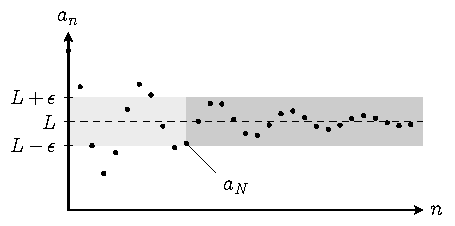
\includegraphics{realanalysis/realsandsequences/convergence.pdf}
  \caption{Convergence of sequences}
  \label{fig:reals-convergence_epsilon}
\end{figure}

\section{Construction of the reals by Dedekind cuts}

The construction of the reals by Dedekind cuts is arguably way simpler than the Cauchy
sequences construction.

\section{Exponentiation}

\section{Existence of \(\e\)}
